%----------------------------------------------------------------------------
\chapter{\Literature}
%----------------------------------------------------------------------------
\section{A vezetés és menedzsment fogalmi elhatárolása}
%----------------------------------------------------------------------------

A „vezetés” és a „menedzsment” kifejezéseket a mindennapokban gyakran szinonimaként használjuk, 
mégis eltérő tartalmakat hordoznak. 
A menedzsment inkább a szervezéshez, tervezéshez és az erőforrások hatékony felhasználásához kapcsolódik, 
míg a vezetés ennél mélyebbre nyúl: az emberek irányításáról, motiválásáról és inspirálásáról szól.
Ahogy Peter Drucker is megfogalmazta: 
„A menedzser a dolgokat jól csinálja, a vezető pedig a jó dolgokat csinálja.” \cite{drucker1954}
A vezető tehát nem pusztán végrehajt, hanem irányt mutat, értéket közvetít és jövőképet ad a csapatnak. 

A modern vezetéselméletek szerint a legjobb vezetők képesek egyensúlyt teremteni a strukturált 
menedzseri gondolkodás és az emberközpontú vezetői szemlélet között \cite{mintzberg1975}. 
A hatékony vezetés így nem csupán a célok elérését jelenti, hanem az emberek fejlődésének támogatását is, 
amely a szervezeti siker egyik legfontosabb tényezője.

%----------------------------------------------------------------------------
\section{A kompetencia fogalma és típusai}
%----------------------------------------------------------------------------

A kompetencia olyan összetett jellemző, amely magában foglalja az egyén tudását, 
készségeit, attitűdjeit és motivációját - vagyis mindazt, ami lehetővé teszi, 
hogy valaki eredményesen lássa el a feladatait \cite{spencer1993}. 
A kompetencia nem veleszületett adottság, hanem folyamatosan fejleszthető és tanulható tulajdonság.

Három fő típusa különíthető el:

\begin{itemize}
    \item \textbf{Szakmai kompetenciák:} a munkakörhöz kapcsolódó technikai ismeretek és gyakorlati készségek.
    \item \textbf{Személyes kompetenciák:} önismeret, döntéshozatal, felelősségvállalás, problémamegoldás.
    \item \textbf{Szociális (személyközi) kompetenciák:} kommunikáció, együttműködés, empátia, vezetői befolyás.
\end{itemize}

A vezetői kompetenciák ezek ötvözetéből épülnek fel, és azt mutatják meg, hogy egy vezető milyen mértékben képes hatékonyan irányítani embereket, motiválni őket és a szervezeti célokat a csapat céljaival összehangolni \cite{boyatzis1982}.
%----------------------------------------------------------------------------
\begin{figure}[H]
	\centering
    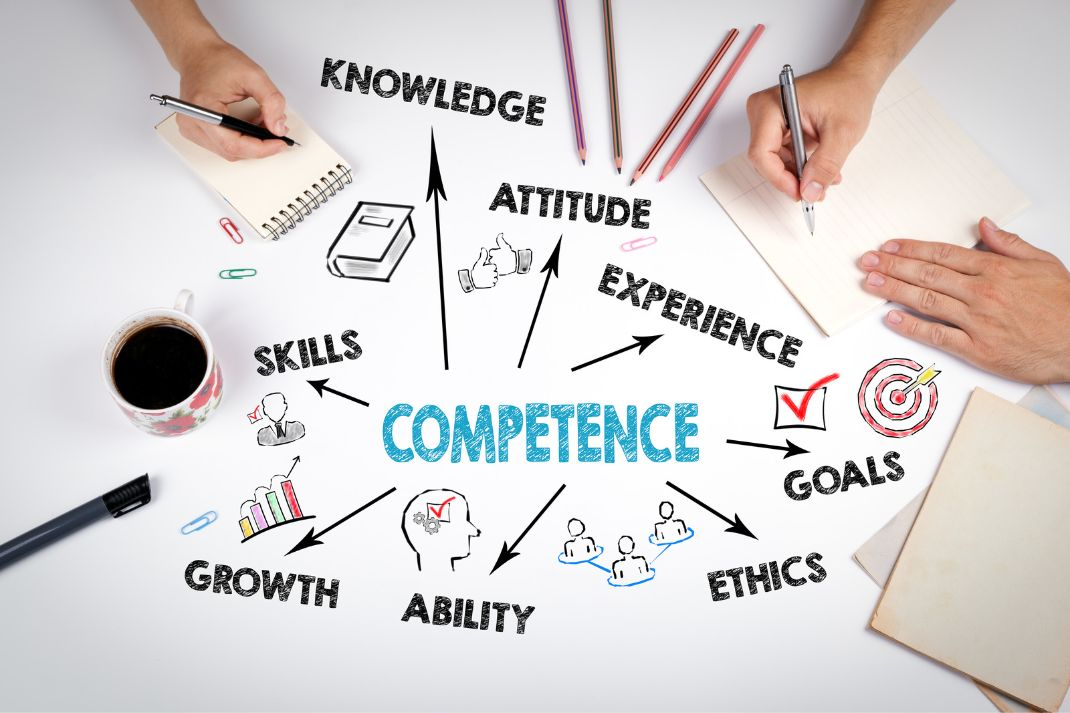
\includegraphics[width=70mm, keepaspectratio]{figures/competence.jpg}
    \caption{Kompetencia típusok vizualizációja} 
    \label {fig:competence}
\end{figure}
%----------------------------------------------------------------------------
\section{A vezetői kompetenciák főbb modelljei}
%----------------------------------------------------------------------------

A vezetői kompetenciák kutatása több évtizedes múltra tekint vissza. 
Robert L. Katz (1955) három alapvető vezetői készséget különített el \cite{katz1955}:

\begin{itemize}
    \item \textbf{Technikai készségek} - a szakmai ismeretek és eszközhasználat képessége.
    \item \textbf{Emberi készségek} - a kommunikáció és együttműködés képessége.
    \item \textbf{Koncepcionális készségek} - a stratégiai gondolkodás, rendszerszintű látásmód.
\end{itemize}

A későbbi modellek, mint például Daniel Goleman érzelmi intelligencia alapú vezetéselmélete, 
kiegészítették ezt azzal, hogy a sikeres vezetés nem csak kognitív képességeken, 
hanem érzelmi tudatosságon, önszabályozáson, empátián és motiváción is múlik \cite{goleman1998}. 

Az európai vezetői kompetenciakeretek (pl. \textit{European Competency Framework for Managers}) 
hangsúlyozzák a felelős döntéshozatalt, az etikus viselkedést, valamint a csapatfejlesztést és innovációt is mint kulcskompetenciákat \cite{ecfm2010}.

Összességében elmondható, hogy a vezetői kompetenciák nemcsak a „mit tudok” szintjén, 
hanem a „hogyan működöm” szinten is meghatározzák a vezető hatékonyságát. 
Egy jó vezető nemcsak irányít, hanem képes inspirálni, példát mutatni és fejlődni önmaga és a csapata érdekében.